\chapter{Medir a massa}\label{ch:g3:measuring-mass}

Na feira: ``Um \omterm{def:g3:measuring-mass:units}{quilograma} de maçãs, por favor!'' O feirante despeja
maçãs no prato até a balança ficar satisfeita. O que exatamente o
freguês pediu --- e como a balança sabe a hora de parar? Com as
\omterm{def:g3:levers-and-scales:lever}{alavancas} e as \omterm{def:g3:levers-and-scales:scale}{balanças de pratos} na nossa caixa de ferramentas,
estamos prontos para \omterm{def:g2:measuring-length:measure}{medir} uma coisa nova: a \omterm{def:g3:measuring-mass:mass}{massa}.

\section{Massa: quanto material}

\begin{definition}[Massa]\label{def:g3:measuring-mass:mass}
A \emph{massa}\index{massa} de uma coisa diz quanto material ela tem.
Quanto mais material, maior a massa --- e com mais \omterm{def:g2:pushes-and-pulls:force}{força} a Terra a
puxa para baixo, e é por isso que as coisas com mais massa parecem
mais pesadas na sua mão e afundam o prato de uma balança.
\end{definition}

\begin{example}[Grande não é pesado]\label{ex:g3:measuring-mass:bignotcheavy}
Um travesseiro enche os seus dois braços e, mesmo assim, você o
carrega fácil. Uma pedra menor que o seu punho cansa o seu pulso. O
travesseiro é grande, mas guarda pouco material --- quase só penas e
\omterm{def:g2:air-around-us:air}{ar}; a pedra é pequena, mas está lotada de material. A \omterm{def:g3:measuring-mass:mass}{massa} é sobre
\emph{quanto material}, e não sobre quanto espaço ele ocupa. (Essas
duas ideias, e a dança complicada entre elas, se reencontram um dia
na história do \omterm{def:g1:floating-and-sinking:words}{flutuar} e do \omterm{def:g1:floating-and-sinking:words}{afundar}.)
\end{example}

\begin{definition}[Grama e quilograma]\label{def:g3:measuring-mass:units}
A \omterm{def:g3:measuring-mass:mass}{massa} é medida em \emph{gramas}\index{grama} (escrito \unit{g}) e
\emph{quilogramas}\index{quilograma} (escrito \unit{kg}):
\[
\qty{1}{kg} = \qty{1000}{g}.
\]
Um clipe de papel tem \omterm{def:g3:measuring-mass:mass}{massa} de cerca de \qty{1}{g}; uma maçã, cerca
de \qty{150}{g}; uma caixa de leite, cerca de \qty{1}{kg}; você,
algumas dezenas de quilogramas. Como o \omterm{def:g2:measuring-length:units}{metro}, essas \omterm{def:g2:measuring-length:measure}{unidades} são as
mesmas para todo mundo na Terra.
\end{definition}

\section{Pesar com uma balança de pratos}

\begin{method}[Pesar com blocos]\label{met:g3:measuring-mass:weigh}
Para \omterm{def:g2:measuring-length:measure}{medir} a \omterm{def:g3:measuring-mass:mass}{massa} de um melão com uma \omterm{def:g3:levers-and-scales:scale}{balança de pratos} e uma caixa
de blocos de metal marcados (\qty{500}{g}, \qty{200}{g},
\qty{100}{g}, \qty{50}{g}, \dots):
\begin{enumerate}
  \item confira se a balança vazia fica na horizontal;
  \item ponha o melão num dos pratos;
  \item acrescente blocos ao outro prato, começando pelos maiores que
        forem úteis, até os pratos ficarem na horizontal;
  \item some os blocos: o total deles é a \omterm{def:g3:measuring-mass:mass}{massa} do melão.
\end{enumerate}
Se os pratos se nivelarem com um bloco de \qty{500}{g}, um de
\qty{200}{g} e um de \qty{100}{g}, a \omterm{def:g3:measuring-mass:mass}{massa} do melão é
$500 + 200 + 100 = \qty{800}{g}$.
\end{method}

\begin{omfigure}
\begin{tikzpicture}[scale=0.85]
  \draw[thick] (5.5,0) -- (5.5,2.6);
  \draw[thick] (4.9,0) -- (6.1,0);
  \draw[very thick] (2.5,2.6) -- (8.5,2.6);
  \fill (5.5,2.6) circle (2.4pt);
  \draw[thick] (2.5,2.6) -- (2.2,1.5) (2.5,2.6) -- (2.8,1.5);
  \draw[thick] (1.9,1.5) .. controls (2.5,1.05) .. (3.1,1.5);
  \draw[thick] (8.5,2.6) -- (8.2,1.5) (8.5,2.6) -- (8.8,1.5);
  \draw[thick] (7.9,1.5) .. controls (8.5,1.05) .. (9.1,1.5);
  \draw[thick, fill=omMeth, fill opacity=0.4] (2.5,1.55) circle (0.42);
  \node[font=\footnotesize] at (2.5,1.55) {melão};
  % all three marked blocks, each with its value
  \draw[thick, fill=omExo, fill opacity=0.4] (8.0,1.2) rectangle (8.55,1.7);
  \node[font=\scriptsize] at (8.28,1.45) {$500$};
  \draw[thick, fill=omExo, fill opacity=0.4] (8.6,1.2) rectangle (8.95,1.5);
  \node[font=\scriptsize] at (8.78,1.35) {$200$};
  \draw[thick, fill=omExo, fill opacity=0.4] (8.1,1.7) rectangle (8.35,1.9);
  \node[font=\scriptsize] at (8.22,1.8) {$100$};
  \node[right, font=\footnotesize, align=left] at (9.35,1.7)
    {$500 + 200 + 100$:\\\qty{800}{g} de blocos};
  \node[below, font=\small] at (5.5,-0.3)
    {pratos nivelados: a massa do melão é igual ao total dos blocos};
\end{tikzpicture}

{\small Pesando o melão: acrescentam-se blocos até os pratos ficarem
nivelados; a soma deles é a resposta.}
\end{omfigure}

\begin{omfigure}
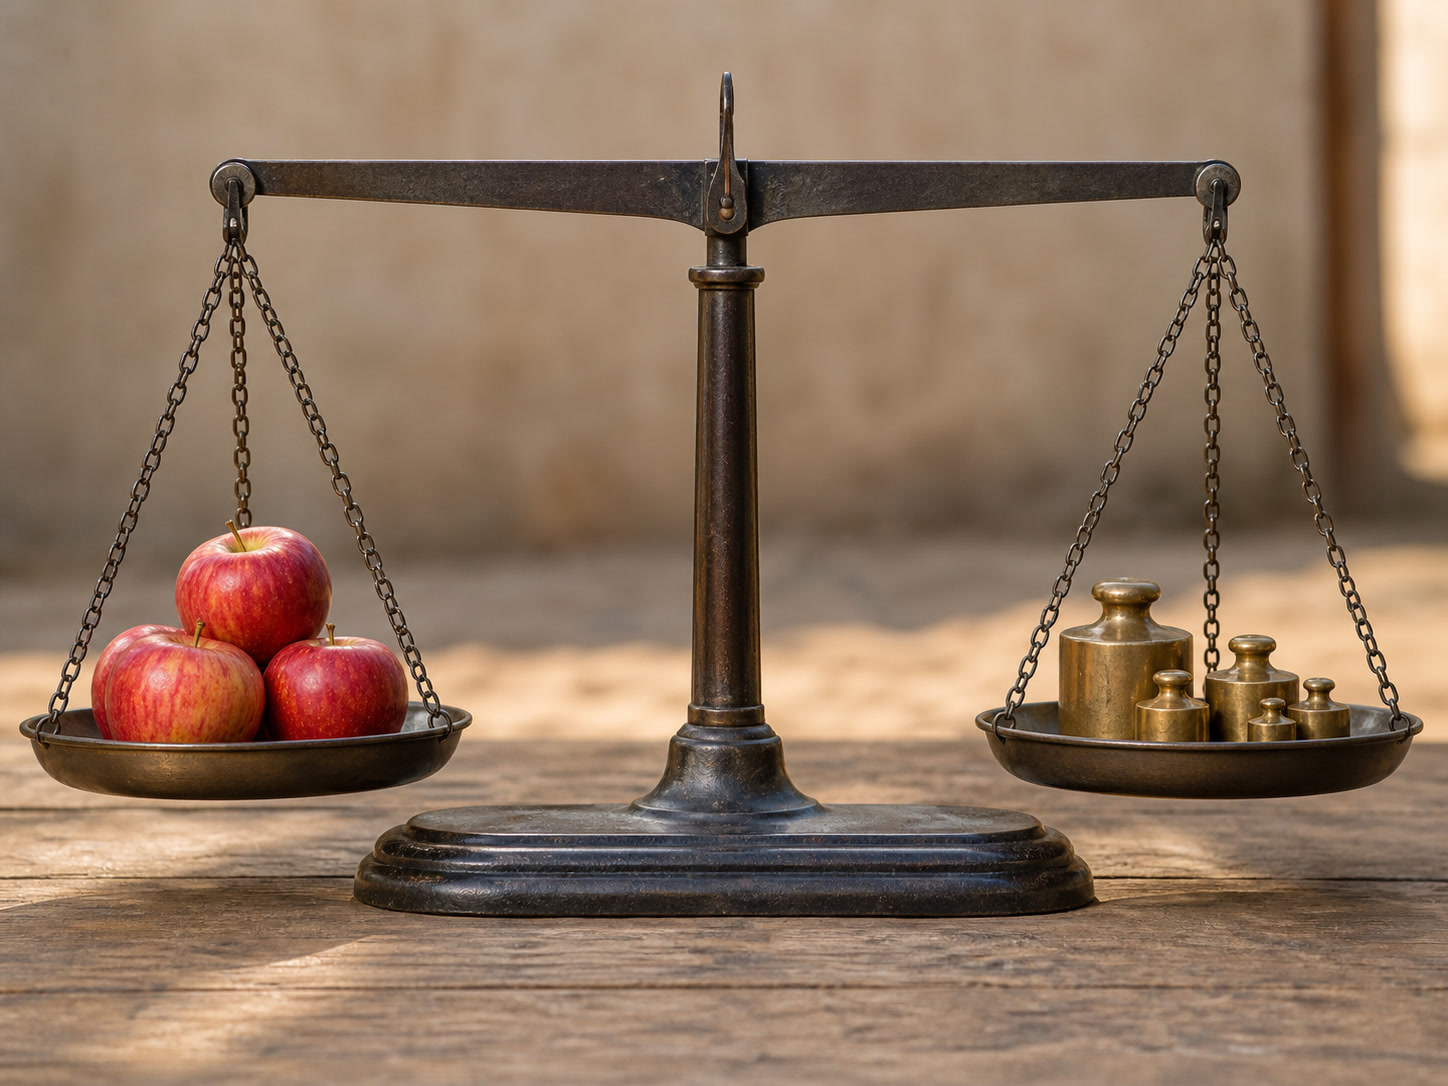
\includegraphics[width=0.52\linewidth]{images/book1/ai/g3-mass-balance-scale.jpg}

{\small Uma \omterm{def:g3:levers-and-scales:scale}{balança de pratos} no seu serviço silencioso: pratos nivelados, então a \omterm{def:g3:measuring-mass:mass}{massa} das maçãs é igual ao total dos pesos de latão.}
\end{omfigure}

\begin{example}[Outras balanças]\label{ex:g3:measuring-mass:otherscales}
A balança de cozinha e a balança de banheiro não têm segundo prato:
você põe a carga em cima e um ponteiro gira (ou um número acende)
para mostrar a \omterm{def:g3:measuring-mass:mass}{massa} diretamente. Lá dentro, uma mola comprimida faz
a comparação por você. Práticas e rápidas --- mas a velha balança de
dois pratos não esconde máquina nenhuma: é só a regra da \omterm{def:g3:levers-and-scales:lever}{alavanca} que
você já entende.
\end{example}

\begin{example}[Lendo a feira]\label{ex:g3:measuring-mass:market}
``Um \omterm{def:g3:measuring-mass:units}{quilograma} de maçãs'' quer dizer: maçãs até a balança equilibrar
um bloco de \qty{1}{kg} --- mais ou menos $6$ ou $7$ maçãs. A farinha
vem em pacotes de \qty{1}{kg}, as barras de chocolate muitas vezes
têm \qty{100}{g}, uma carta precisa de cerca de \qty{20}{g} de papel,
e a regra do carteiro ``abaixo de \qty{20}{g}, um selo'' é uma regra
de \omterm{def:g3:measuring-mass:mass}{massa}.
\end{example}

\section{A massa acompanha o material}

\begin{proposition}[Mesmo material, mesma massa]\label{prop:g3:measuring-mass:conserved}
Mudar o \emph{formato} de uma coisa não muda a \omterm{def:g3:measuring-mass:mass}{massa} dela. Enrole uma
bola de \omterm{def:g3:measuring-mass:mass}{massa} de pão até virar uma cobrinha, achate-a numa panqueca
ou corte-a em quatro e pese todos os pedaços juntos: a balança
informa a mesma \omterm{def:g3:measuring-mass:mass}{massa} toda vez. A \omterm{def:g3:measuring-mass:mass}{massa} conta o material --- e
amassar, enrolar e cortar não acrescentam nem tiram material nenhum.
\end{proposition}

\begin{omfigure}
\begin{tikzpicture}[scale=0.85]
  \draw[thick, omDef!70!black, fill=omDef, fill opacity=0.5]
    (1.3,1.0) circle (0.55);
  \node[below, font=\small, align=center] at (1.3,0.15)
    {uma bola de massa:\\\qty{300}{g}};
  \draw[thick, omDef!70!black, fill=omDef, fill opacity=0.5]
    (6.2,0.85) ellipse (1.5 and 0.28);
  \node[below, font=\small, align=center] at (6.2,0.15)
    {enrolada em cobrinha:\\\qty{300}{g}};
  \draw[thick, omDef!70!black, fill=omDef, fill opacity=0.5]
    (9.55,0.75) circle (0.3);
  \draw[thick, omDef!70!black, fill=omDef, fill opacity=0.5]
    (10.28,0.75) circle (0.3);
  \draw[thick, omDef!70!black, fill=omDef, fill opacity=0.5]
    (9.72,1.32) circle (0.28);
  \draw[thick, omDef!70!black, fill=omDef, fill opacity=0.5]
    (10.4,1.32) circle (0.28);
  \node[below, font=\small, align=center] at (10.0,0.15)
    {quatro pedaços juntos:\\\qty{300}{g}};
\end{tikzpicture}

{\small Um pedaço de \omterm{def:g3:measuring-mass:mass}{massa}, três formatos --- e uma única \omterm{def:g3:measuring-mass:mass}{massa}. A
balança nunca se engana com uma mudança de formato.}
\end{omfigure}

\begin{remark}[A balança ignora as aparências]\label{rem:g3:measuring-mass:appearances}
Esse é o poder silencioso de \omterm{def:g2:measuring-length:measure}{medir}: os olhos julgam uma panqueca
achatada ``maior'' que a bola de onde ela veio, e um travesseiro
fofinho ``mais pesado'' que uma pedra --- mas a \omterm{def:g3:levers-and-scales:scale}{balança de pratos},
como o \omterm{def:g3:temperature-thermometers:temperature}{termômetro} e a régua antes dela, informa o material e nada
mais. Um a um, os nossos instrumentos vão trocando o ``parece'' pelo
``é''.
\end{remark}

\section{Exercícios}

\begin{exercise}[$\star$]\label{exo:g3:measuring-mass:1}
O que a \omterm{def:g3:measuring-mass:mass}{massa} de uma coisa diz? Quais duas \omterm{def:g2:measuring-length:measure}{unidades} a medem, e
quantos \omterm{def:g3:measuring-mass:units}{gramas} cabem num \omterm{def:g3:measuring-mass:units}{quilograma}?
\end{exercise}

\begin{exercise}[$\star$]\label{exo:g3:measuring-mass:2}
Escolha a \omterm{def:g3:measuring-mass:mass}{massa} mais provável: um clipe de papel --- \qty{1}{g} ou
\qty{1}{kg}? Uma maçã --- \qty{150}{g} ou \qty{15}{kg}? Uma caixa de
leite --- \qty{1}{g} ou \qty{1}{kg}? Um gato --- \qty{4}{kg} ou
\qty{400}{kg}?
\end{exercise}

\begin{exercise}[$\star$]\label{exo:g3:measuring-mass:3}
Os pratos se nivelam com uma abóbora de um lado e um bloco de
\qty{500}{g} mais dois blocos de \qty{200}{g} do outro. Qual é a
\omterm{def:g3:measuring-mass:mass}{massa} da abóbora?
\end{exercise}

\begin{exercise}[$\star$]\label{exo:g3:measuring-mass:4}
Por que a balança vazia precisa ficar na horizontal antes de qualquer
pesagem? (Lembre do comerciante trapaceiro.)
\end{exercise}

\begin{exercise}[$\star$]\label{exo:g3:measuring-mass:5}
Uma bola de praia é muito maior que uma lata de sopa e, mesmo assim,
é a lata que \omterm{def:g1:floating-and-sinking:words}{afunda} o prato. Explique com o
\cref{ex:g3:measuring-mass:bignotcheavy}.
\end{exercise}

\begin{exercise}[$\star$]\label{exo:g3:measuring-mass:6}
Quantos \omterm{def:g3:measuring-mass:units}{gramas} há em \qty{2}{kg}? E em meio \omterm{def:g3:measuring-mass:units}{quilograma}? Qual é mais:
\qty{1200}{g} ou \qty{1}{kg}?
\end{exercise}

\begin{exercise}[$\star$]\label{exo:g3:measuring-mass:7}
Uma barra de chocolate de \qty{100}{g} é quebrada em todos os seus
quadradinhos, e todos os quadradinhos vão juntos para a balança. Que
\omterm{def:g3:measuring-mass:mass}{massa} a balança mostra, e qual lei diz isso?
\end{exercise}

\begin{exercise}[$\star$]\label{exo:g3:measuring-mass:8}
A balança de cozinha e a balança de dois pratos pesam as duas um
pacote de farinha. O que cada uma usa para fazer a comparação --- e
qual delas funciona por uma regra que você aprendeu três capítulos
atrás?
\end{exercise}

\begin{exercise}[$\star$]\label{exo:g3:measuring-mass:9}
A padeira precisa de \qty{800}{g} de farinha e tem blocos de
\qty{500}{g}, \qty{200}{g}, \qty{200}{g}, \qty{100}{g} e
\qty{50}{g}. Encontre duas maneiras diferentes de pesar exatamente
\qty{800}{g} --- sabendo que os blocos podem ficar em
\emph{qualquer} um dos pratos.
\end{exercise}

\begin{exercise}[$\star\star$]\label{exo:g3:measuring-mass:10}
Nina pesa uma laranja inteira: \qty{200}{g}. Ela descasca a laranja e
pesa só a laranja descascada: \qty{160}{g}. A
\cref{prop:g3:measuring-mass:conserved} falhou? Onde estão os \omterm{def:g3:measuring-mass:units}{gramas}
que sumiram, e como Nina poderia provar isso com mais uma pesagem?
\end{exercise}

\begin{exercise}[$\star\star$]\label{exo:g3:measuring-mass:11}
Uma charada, enfim fácil para você: o que tem mais \omterm{def:g3:measuring-mass:mass}{massa}, um
\omterm{def:g3:measuring-mass:units}{quilograma} de penas ou um \omterm{def:g3:measuring-mass:units}{quilograma} de ferro? E o que ocupa mais
espaço? Explique por que tanta gente responde errado à primeira
pergunta.
\end{exercise}
